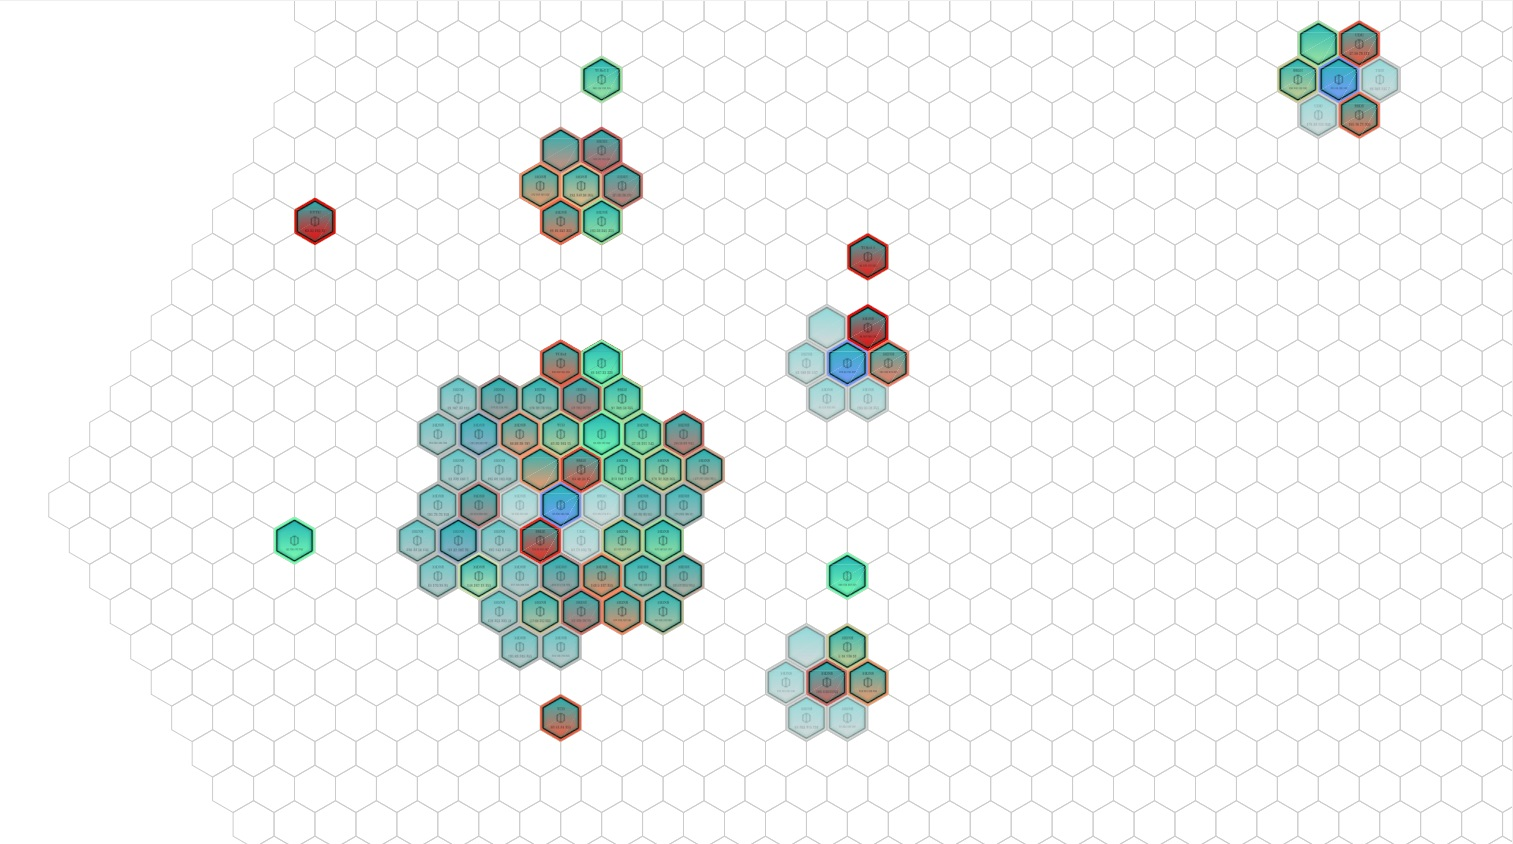
\includegraphics[width=\linewidth]{materials/groups.jpg}
Acting on the hexagonal grid, this visualization puts to use two important visual factors:
size and proximity.

As the traffic in the network arises, the visualization groups together all the machines
sending packets to a one specific other device. As more and more machines communicate with a specific
address, more and more nodes appear around the hexagon representing that destination.

The colour of the communicating nodes represents how much data they send. More heavily used destinations 
will thus have more orange and red nodes around them, and destinations used by a lot of machines will have a greater number of nodes around them. Therefore, both the size of the segment and its color transmit important information.

The placement of the nodes is automatic. The procedure employed always assures that there is enough space around a center
and that no two nodes overlap.

This visualization helps detecting the machines that perform a server role in the network.
It also allows a user to quickly guess what type of service the device is providing. Each node specifies the
most commonly used protocol, thus revealing the possible role of the server node.